\documentclass[11pt,french]{report}
\usepackage[utf8]{inputenc}
\usepackage[hidelinks]{hyperref}
\usepackage{babel}
\usepackage[T1]{fontenc}
\usepackage{graphicx}
\graphicspath{{./graphics/}}
\usepackage{titlesec}

\titleformat{\chapter}[display]{\normalfont\bfseries}{}{0pt}{\Huge}

% \newcommand\sectionbreak{\clearpage}

\title{Comment découvrir son corps ?}
\author{Lucas Schwab}
\date{Mars - Aout 2020}

\begin{document}

\maketitle

% Le rapport décrit le travail effectué pendant le stage, tout en le plaçant dans son contexte.  Typiquement on s’attend à un rapport d'une taille entre 30 et 40 pages en utilisant une police de caractères de 11 points, sans compter les éventuelles annexes et les pages avant l’introduction.

% L'introduction doit présenter brièvement  

%     le sujet de stage tel que formulé initialement,
%      les modifications opérées pendant le stage,
%      les résultats obtenus pendant le stage.

% Cette partie doit être assez courte, le tout sera expliqué plus en détail dans les chapitres suivants qui doivent décrire 

%     le cadre de travail, le descriptif de l’entreprise/le laboratoire
%     le sujet et son contexte 
%     le travail réalisé (résultats obtenus, démarche et méthode suivies, difficultés rencontrées, planning, ...)
%     les conclusions.

% Il faut également fournir la liste des références bibliographiques consultées pendant le stage.  Les références doivent être aussi complètes que possible et citées dans le corps du rapport.

% Un soin particulier devra être accordé à l'orthographe, la grammaire, et la typographie.

\tableofcontents

%%%%%%%%%%%%%%%%%%%
% % % SECTION % % %
%%%%%%%%%%%%%%%%%%%
\chapter{Remerciements}

Je tiens à remercier mes tuteurs de stage, Mr Amine BOUMAZA et Mr Alain DUTECH, enseignants-chercheurs dans l'équipe LARSEN pour leur accompagnement et les précieux conseils qu'ils m'ont donnés.

Je remercie également ma tutrice Mme Isabelle DEBLED-RENNESSON pour m'avoir suivi tout au long de ce stage, ainsi que tous mes professeurs pour les enseignements qu'ils m'ont donné.

Je tiens à remercier toutes les personnes qui ont contribué à mon stage et qui m'ont aidé lors de la rédaction de ce rapport.

% Je tiens à remercier en premier lieu l’entreprise CapGemini, pour avoir accepté de me prendre pour ce stage, et plus particulièrement mes tuteurs de stage Pierre CHIRIOT et Romain RUEZ, pour leur accompagnement tout au long de ce projet et pour les précieux conseils qu’ils m’ont donnés.
% Je remercie également ma tutrice à l’université, Phuc NGO, pour m’avoir suivi tout au long de ce stage, ainsi que Horatiu CIRSTEA pour ses enseignements pendant ces deux dernières années.
% Enfin, je remercie évidemment mon père, grâce à qui ce rapport ne contient aucune faute d’orthographe, de grammaire, ou de syntaxe. Si cette lecture vous est agréable, c’est en partie grâce à lui


% \underline{Exemple d'une ancienne stagiaire}\\[10pt]
% Je tiens à remercier toute personne ayant participé de près ou de loin à ce stage.\\[10pt]
% Tout d’abord mon tuteur,  Monsieur  Boumaza Amine pour m’avoir aiguillé,  accompagné  et  pour avoir répondu à mes questions.\\[10pt]
% Le LORIA et Monsieur Marion Jean-Yves pour avoir accepté mon stage au sein du laboratoire.\\[10pt]
% L’équipe LARSEN et Monsieur Charpillet François pour avoir accepté mon stage au sein de son équipe.\\[10pt]
% Mon enseignant référent, Madame Souquières Jeanine pour avoir été là si j’avais un problème.\\[10pt]
% L’Institut  des  Sciences  du  Digital  Management  et  Cognition, Monsieur  Thomann  Laurentet les personnes ayant contribué à la partie administrativede ce stage.\\[10pt]
% Toutes les personnes m’ayant aidé lors de la recherche de ce stage et pendant toute la durée de ce dernier.


%%%%%%%%%%%%%%%%%%%
% % % SECTION % % %
%%%%%%%%%%%%%%%%%%%
\chapter{Introduction}
% le sujet de stage tel que formulé initialement
\section{Sujet}

\noindent\textbf{Motivations}

Apprendre à contrôler un robot redondant, c’est-à-dire un robot où plusieurs configurations permettent d’atteindre une position donnée, reste une tâche difficile en Intelligence Artificielle. Elle est d’autant plus difficile quand on ne dispose pas de modèle du robot. Le but de ce projet est d’explorer différentes approches pour apprendre de manière autonome ce type de contrôle.\\[10pt]
\noindent\textbf{Sujet \& Cadre du travail}

Ce projet rentre dans le cadre général de l’apprentissage artificiel et plus précisément dans le cadre où l’agent apprenant ne dispose par d’un modèle (cinématique et dynamique) de son corps. Il doit “apprendre” ce modèle en observant les effets de ses différentes actions de manière progressive, à l’image des nouveaux nés, dont les premiers gestes sont assez imprécis et s’affinent au fur et à mesure du développement de l’enfant et la découverte de leur corps.

Plusieurs algorithmes d’apprentissage proposent d’imiter le développement chez les enfant en s’appuyantsur un processus exploratoire des espaces sensoriels et moteur du robot. L’objectif du travail de recherche proposé est de proposer et d’implanter un algorithme d’exploration des effets des action moteur surun robot réel.\\[10pt]
Le protocole expérimental envisagé s’appuiera sur un robot ErgoJr à plusieurs degrés de liberté. Une caméra sera installée en bout de bras. Les algorithmes d’apprentissage devront permettre de mettre en œuvre des tâches d’asservissement visuel (parexemple, suivre “du regard” un stimulus visuel).


% les modifications opérées pendant le stage
\section{Travail apporté}

Nous proposons d’articuler ce projet en plusieurs étapes.
\begin{itemize}
    \item Étude bibliographique sur les méthodes de la littérature permettant le type d’apprentissage visé dans ceprojet. Cette étude pourrait être amorcée par la thèse.
    \item Mise au point d’un algorithme et expérimentations pour tests et validations.
\end{itemize}

% les résultats obtenus pendant le stage
\section{Résultats obtenus}

% Afficher une démonstration sur robot réel

%%%%%%%%%%%%%%%%%%%
% % % SECTION % % %
%%%%%%%%%%%%%%%%%%%
% le cadre de travail, le descriptif de l’entreprise/le laboratoire
\chapter{Cadre de travail}

% Le Loria, Laboratoire lorrain de Recherche en Informatique et ses Applications est une Unité Mixte de Recherche (UMR 7503), commune à plusieurs établissements : le CNRS, l’Université de Lorraine et Inria.
% Depuis sa création en 1997, le Loria a pour mission la recherche fondamentale et appliquée en sciences informatiques.
% Le Loria est membre de la Fédération Charles Hermite qui regroupe les trois principaux laboratoires de recherche en mathématiques et STIC (science et technologies de l’information et de la communication) de Lorraine. Le laboratoire fait partie du pôle scientifique AM2I (Automatique, Mathématiques, Informatique et leurs interactions) de l’Université de Lorraine.
% Nos travaux scientifiques sont menés au sein de 29 équipes structurées en 5 départements, dont 15 sont communes avec Inria, représentant un total de plus de 400 personnes. Le Loria est un des plus grands laboratoires de la région lorraine.



% \underline{Exemple d'une ancienne stagiaire}\\[10pt]
% Depuis 1976, le laboratoire du CRIN (Centre de Recherche en Informatique de Nancy) regroupe des chercheurs dont les problématiques se trouvent autour de deux axes: Théorie et Techniques du Logiciel (TTL) et Reconnaissance des Formes et Intelligence Artificielle (RFIA).
% Le rapprochement de l’INRIA, du CRIN et du CNRS a permis le développement de trois autres secteurs pluridisciplinaires: l’informatique et les sciences humaines et sociales, la modélisation et le calcul à hautes performances et les sciences de la vie et de la santé.
% C’est suite à tout cela que le Laboratoire lorrain de Recherche en Informatique et ses Applications (LORIA) a été créé en 1997. Il s’agit d’une Unité Mixte de Recherche (UMR) commune au CNRS, à l’Université de Lorraine et à l’INRIA. Il a pour directeur Jean-Yves Marion et Yannick Toussaint comme directeur adjoint.
% Il est composé de 30 équipes (dont 15 communes avec l’Inria), elles-mêmes structurées en 5 départements (Figure 4).
% Le 5ème département («Systèmes complexes, intelligence artificielle et robotique») est composé de 5 équipes: BISCUIT, KIWI, CAPSID, LARSEN et NEURORYTHMS. Son objectif est l’étude des systèmes complexes et leurs interactions, de l’intelligence artificielle et de la robotique.
% Ce stage se déroule au sein de l’équipe LARSEN (anciennement MaIA) qui a été créée au premier janvier 2015 et qui a pour responsable François Charpillet. Cette équipe a pour objectif de faire évoluer des robots en dehors des laboratoires ou des chaines de production.Il faut donc qu’ils puissent interagir (avec des êtres humains et d’autres robots) et être autonomes (s’adapter à des changements de leur environnement ou de leur morphologie).

%%%%%%%%%%%%%%%%%%%
% % % SECTION % % %
%%%%%%%%%%%%%%%%%%%
% le sujet et son contexte 
\chapter{Présentation du stage}

%%%%%%%%%%%%%%%%%%%
% % % SECTION % % %
%%%%%%%%%%%%%%%%%%%
% le travail réalisé (résultats obtenus, démarche et méthode suivies, difficultés rencontrées, planning, ...)
\chapter{Travail réalisé}

L'étude de la biologie afin de créer des machines et des robot représente une part importante dans la recherche. Le contexte de ce stage est de s'inspirer des processus dévelopmentaux des systèmes biologiques afin de les reproduire sur des robots. Nous créons ainsi des robots qui ont une enfance et qui basent leurs décisions sur l'éxpérience acquise au cours du temps. Pour la suite, j'utiliserais seulement un bras robotique, qui peut être n'importe quel suite de moteurs prenant une certaine position, un angle, reliés par des sections rigides. Le but est de controller un robot en lui donnant une position à atteindre.

En connaissant la forme des sections rigides et l'angle pris par chacun des moteurs, il est assez facile d'estimer la position de l'effecteur du robot, le bout de son bras. Ceci est la modélisation géométrique directe. Il suffit d'appliquer quelques rotations et translations sur une matrice. Mais même cette méthode possède des limites. En effet, si le robot possède des sections flexibles, ou si l'environnement dans lequel il évolue est compliqué, il devient très difficile d'appliquer une modélisation géométrique directe. Mais ce qui nous interesse ici n'est pas de trouver la position de l'effecteur à partir d'une posture, mais plutot de trouver une posture pour atteindre une certaine position. Ceci est la fonction de la modélisation géométrique inverse. Elle est cependant très compliquée à appliquer même à un robot ne possédant que des sections rigide et évoluant dans un environnement simple. La redondance, le fait que le robot peut atteindre une position avec plusieurs posture différentes, est déjà un problème difficile à résoudre. C'est pour cela qu'une autre méthode a été étudiée pendant ce stage.

Nous n'essayons pas de créer une modélisation géométrique inverse, ce qui doit être fait pour chaque robot spécifiquement, mais en s'inspirant du développement d'un système biologique, le robot peut être contrôlé grâce à l'expérience qu'il a acquis. Le principe est simple : donner un maximum d'expérience au robot pour qu'il puisse ensuite construire son propre modèle inverse. Il est possible d'appliquer ce raisonnement qu'avec des observations dans le monde réel, rendant ainsi inutile la mise en place d'une modélisation géométrique et cinématique directe.

\section{Motor Babling}

Une première approche pour que le robot acquière de l'expérience est une exploration de ses espaces moteurs et sensoriels. Ceci est comparable au comportement d'un nouveau né qui ne contrôle pas ses mouvements. Le robot va prendre une posture totalement aléatoire et observer en résultat la position de son effecteur dans le monde. Ceci est un babillage moteur (ou motor babling en anglais). Nous construisons ainsi un catalogue, contenant toutes les postures essayées et les observations associées, ce qui constitue la mémoire et l'expérience du robot.

\section{Nearest Neighbor}

Une fois que le catalogue contenant les commandes et les observations est construit, il faut pouvoir l'utiliser pour atteindre des positions demandées. La première manière pour trouver une commande à executer afin d'aller à une position donnée est de prendre l'observation dans le catalogue la plus proche du but et d'appliquer la posture associée. Il est donc indispensable d'avoir un algorithme pour trouver le plus proche voisin efficacement pour avoir un résultat rapidement. Il existe des structure de données comme le KDTree qui partitionne l'espace pour stocker les points et permet une recherche du plus proche voisin plus rapide qu'avec un simple tableau. 

Il y a cependant plusieurs contraintes à appliquer à ce plus proche voisin, ou Nearest Neighbor en anglais, la recherche rapide étant la première. Si nous voulons pouvoir utiliser le catalogue dans un environnement continue, il nous faut une infinité de points dans celui-ci afin de couvrir entièrement l'espace. Une autre solution est aussi de rechercher plusieurs points les plus proches du but, et de renvoyer une posture résultant de la moyenne de toutes les postures trouvées, pondéré par la distances des observations au but. De cette façon il est possible de couvrir un espace continue avec un nombre fini de points dans le catalogue.

Une troisième contrainte au Nearest Neighbor, autre que la recherche rapide et la recherche de plusieurs plus proches voisins, est la possibilité d'ajouter des données dans le catalogue pendant l'utilisation. Ceci est impossible avec le KDTree qui ne peut garantir un équilibre dans la structure de donnée si des points sont ajoutés en cours d'utilisation. C'est pourquoi j'utilise une structure appellée RTree. Cette structure est en forme d'arbre, où chaques points proches sont représentés par un rectangle englobant au niveau supérieur de l'arbre. RTree permet ainsi l'insertion facile de donnée sans dégrader le temps de recherche d'un plus proche voisin.

\section{goal babling}

L'exploration de l'espace des moteurs du robot ne remplis pas toujours efficacement le catalogue, et il est possible de diriger l'apprentissage en choisisant des but à atteindre. C'est donc un babillage par but, ou Goal Babling en anglais. La selection d'un but est importante sur la qualité du catalogue résultat. Si le robot est complexe et que le Motor Babling n'explore pas assez l'espace de travail, la selection de but peut forcer cette exploration. Cependant, si tous les buts générés sont mal positionnés, le catalogue perdra en précision d'execution. Il existe plusieurs façon de générer un but.

\subsection{Agnostic Goal Generation}

Générer un but aléatoirement est facile, il suffit de générer uniformément des coordonnées dans un espace défini. Les buts sont générées sans aucune connaissance au préalable sur le robot, c'est donc une génération de but agnostique. Afin de pouvoir gérer le taux d'exploration avec cet algorithme, les positions extrêmes rencontrées lors de l'apprentissage, le minimum et maximum atteint sur chacun des axes, sont enregistrés. Cela donne une zone que le robot pourrais atteindre. Un but sera généré dans cette zone, dont la taille a été mutlipliée par un facteur, qui déterminera ainsi le taux d'exploration.

Cependant cette méthode est assez limitée, surtout que l'espace de travail n'est que rarement proche d'un cube (ou d'un pavé droit).

\subsection{Goals on Grid}

Afin d'approcher l'espace de travail du robot sans avoir de connaissance sur celui-ci, il est possible de partitionner l'espace en une grille. Lors de l'apprentissage, toutes les cellules atteintes par les observations du catalogue sont enregistrée, ce qui nous donne une estimation sur l'espace atteint. Gérer le taux d'exploration ou d'exploitation est donc facile, pour augmenter l'exploitation et la précision, il suffit de générer un but dans une cellule déjà atteinte. Pour augmenter l'exploration et la couverture, il faut générer un but dans une cellule non atteinte. 

\subsubsection{Frontier}

L'algorithme frontier permet de selectionner une cellule non atteinte mais potentiellement atteignable. Premièrement, une observation dans le catalogue est selectionnée. Ensuite, une direction est générée aléatoirement. L'algorithme parcour ensuite la grille à partir de l'observation en suivant la direction jusqu'à rencontrer une cellul qui n'est pas encore atteinte. Cette cellule est donc à la frontière de la zone atteinte par le robot. L'algorithme Frontier permet donc d'explorer un espace plus proche de l'espace de travail que l'algorithme Agnostic.


\chapter{Observations}

\section{Mesures}

Afin de pouvoir comparer différents algorithmes, je vais mesurer la couverture du catalogue réalisé ainsi que la précision du résultat.

\subsection{Couverture}

La couverture sera mesurée à partir de ces deux valeurs:

\begin{itemize}
    \item[$\bullet$] Le volume, qui correspond au volume de l'enveloppe convexe des points du catalogue. Cela permet de mesurer la taille de l'espace couvert par l'algorithme et déterminer un taux d'exploration.
    \item[$\bullet$] Le remplissage, qui est le ratio entre le nombre de cellules de la discretisation de l'espace populées par les points du catalogue et le nombre de cellules théoriquement atteignables, comme par exemple les cellules dans une sphère dont le rayon est la taille du bras robotique. Cela permet de mesurer le taux de remplissage de l'espace couvert.
\end{itemize}

\subsection{Precision}

La précision sera déduite à partir de l'erruer, qui est la distance entre un but donné et l'observation générée par le résultat du modèle inverse. Les mêmes buts seront utilisés pour comparer tous les algorithmes. Deux listes de but ont été retenues:

\begin{itemize}
    \item[$\bullet$] La première contient des buts générés uniformément dans un espace théoriquement atteignable par le robot. L'espace selectionné est 3/4 d'une demi-sphère. Il est inutile de demander le robot d'atteindre une zone sous sa base, il ne peut pas traverser une table, cela enlève une demi-sphère. Nous ne demandons pas au robot d'essayer d'atteindre une zone "derrière lui", ce qui exclue 1/4 de la zone restante. Voir figure \ref{fig:goal_list} pour une représentation du dessus et de face.
    
    \begin{figure}
        \centering
        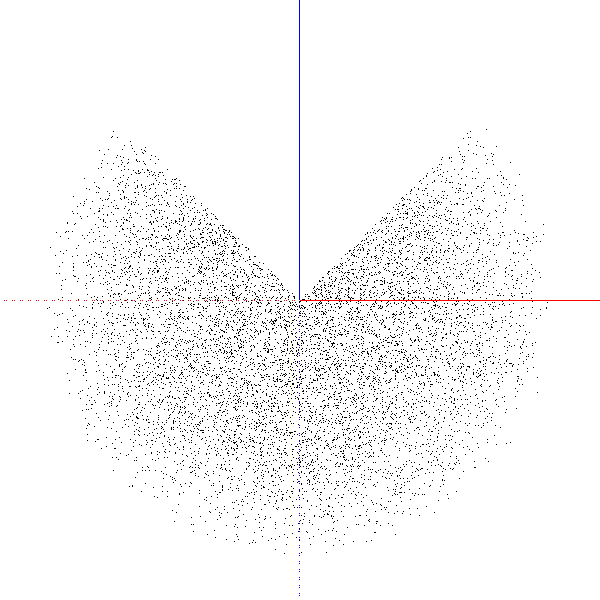
\includegraphics[width=178pt]{goal_list_top} 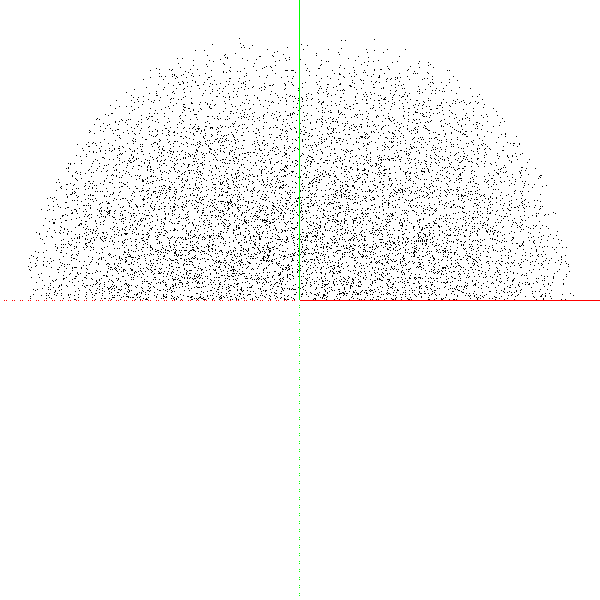
\includegraphics[width=178pt]{goal_list_front}
        \caption{Liste de buts théoriquement atteignables}
        \label{fig:goal_list}
    \end{figure}
    
    \item[$\bullet$] La deuxième contient les observations faites après utilisation de la bibliothèque Ikpy qui contient un modèle inverse. Cette liste ne contient que des observations, donc des point qui sont réellement atteignable. Avec ce modèle inverse il est possible de comparer l'efficacité d'un modèle inverse existant, ici Ikpy, avec le modèle inverse généré par les algorithmes.
\end{itemize}

\section{Paramètres}

Il existe plusieurs paramètres aux différents algorithmes utilisés. Afin de pouvoir les comparer, il faut d'abord trouver les paramètres les plus optimisés pour chacune des instances. L'apprentissage se résume à remplir de la manière la plus efficace possible un catalogue qui représente la vie d'un robot. Un paramètre commun à tous ces apprentissage est donc la taille du catalogue. On peut facilement imaginer qu'un catalogue plus grand permet d'avoir une meilleure précision et une meilleure couverture de l'espace. Deux valeurs de ce paramètre ont étées testées pour ne pas avoir un nombre trop important de version à tester. Afin de vérifier l'hypothèses, ces deux paramètres sont 1 000 entrées dans le catalogue pour représenter une borne inférieure, ainsi que 100 000 entrées dans le catalogue.

\subsection{Motor Babling}

\'A chaque étape du Motor Babling, une posture est choisie en donnant un angle aléatoire à chacun des moteurs généré uniformément sur leur portée. C'est une exploration de tout l'espace moteur du robot, donc tout point atteignable par ce robot possède donc une probabilité non nul d'être dans le catalogue. J'en déduis que la couverture du Motor Babling augmente avec la taille de son catalogue.

Plus il y a de points dans ce catalogue, la distance entre un but et les points du catalogue utilisés dans l'interpolation sera petite, donc la précision de l'algorithme augmente aussi avec la taille de son catalogue.

\subsection{Goal Babling}

Quelque soit l'algorithme de génération du but, pour initier le Goal Babling il faut exécuter un certain nombre d'étape de Motor Babling. C'est donc un paramètre à prendre en compte. Comme il faut commencer par un certain nombre d'étapes de Motor Babling, la borne inférieure testée pour ce paramètre est une proportion de 0.01 étapes sur le nombre total d'entrée du catalogue. Si la proportion est trop grande, cela reviens à faire simplement du Motor Babling. La deuxième valeur testée pour ce paramètre sera donc une proportion de 0.2 sur le nombre total d'entrée du catalogue.

Lorsqu'un but est choisi, une nouvelle entrée dans le catalogue est crée à partir d'une perturbation de donnée existante. Cette perturbation est un autre paramètre à prendre en compte pour du Goal Babling. Avec une perturbation plus elevée, la posture générée sera normalement plus loin de la posture selectionnée. La couverture d'un algorithme augmente donc avec la perturbation. Cependant, l'observation de la posture générée a plus de chance d'être distante du but demandé, et donc la perturbation peut déteriorer la précision de l'algorithme. Les valeurs utilisées pour ce paramètre sont une proportion de 0.05 de la portée du moteur, ainsi qu'une proportion de 0.2 de la portée du moteur.

\subsection{Agnostric Goal Generation}

La génération de but agnostique utilise une zone qui est calculée à partir de la zone couverte par les observations du catalogue. Afin d'ajouter un taux d'exploration à l'algorithme, la zone de génération des buts sera une extension de la zone couverte par le catalogue. Plus le coefficient d'extension est grand, plus la zone dans laquelle les buts sont générés sera grande. Plus le coefficient est grand, plus la zone de génération de but est grande, or le nombre d'entrée du catalogue ne change pas. Ce coefficient impacte donc positivement la couverture mais négativement la précision. Deux valeurs sont utilisées pour ce paramètre. La première est de 0.7, une borne inférieur qui permet d'illustrer si un autre paramètre impacte plus l'exploration que celui-ci. La deuxième est 1.4, valeur supposée non extrême: une valeur trop grande donne une génération de but impossible à atteindre. Le robot se forcerait à n'atteindre que les extrémités de son espace de travail.

\subsection{Frontier Goal Generation}

Lors de l'utilisation du Frontier Goal Generator, ou plus largement du Goals on Grid, il existe un coefficient d'exploration p. Avec une probabilité p l'algorithme va choisir d'explorer l'espace, et avec une probabilité p-1, l'alogirthme choisi d'exploiter le catalogue. Trois valeurs de p ont étées testées. Les dornes 0.01 et 0.9, ainsi qu'une valeur intermédiaire 0.5.

Il est aussi possible de changer la taille d'une cellule pour l'utilisation de Goals on Grid. Une taille de cellule plus petite représentera plus présicemment la zone atteinte par le catalogue, mais rendra l'exploration de l'espace plus lente. Une taille de cellule trop grande et l'algorithme devient une simple génération agnostique. J'ai choisi de fixer la taille de l'espace, et je détermine la taille d'une cellule à partir d'un certain nombre de division de cet espace. Deux valeurs pour ce paramètre ont été testée: 10 divisions (ce qui reviens à des cellules de tailles de 10cm³), et 1 000 divisions (ce qui reviens à des cellules de 1mm³).

%%%%%%%%%%%%%%%%%%%
% % % SECTION % % %
%%%%%%%%%%%%%%%%%%%
% les conclusions
\chapter{Conclusion}


\end{document}
